%
% bezier.tex
%
% (c) 2020 Prof Dr Andreas Müller, Hochschule Rapperswil
%

\subsection{Bézier-Kurven und Splines in der Ebene
\label{buch:subsection:bezier}}
Spline-Interpolation kann auch verwendet werden um Kurven in der Ebene
oder im Raum zu approximieren.
In der Computergraphik ist dabei besonders wichtig, dass sich Kurvenpunkte
mit einfachen Operationen aus einer kleinen Zahl von Parametern berechnen
lassen, damit sie zum Beispiel von einem Graphikprozessor berechnet
werden können.
Dieser Abschnitt soll daher den Zusammenhang zwischen Bézier-Kurven und
Splines aufzeigen.


\subsubsection{Kurven in der Ebene}
Eine Kurve in der Ebene ist eine Abbildung
\[
\gamma \colon \mathbb R \to \mathbb R^2 : t \mapsto \gamma(t) = (x(t),y(t)),
\]
genannt die Parameterdarstellung der Kurve.
Man kann sich den Parameter $t$ als die Zeit vorstellen und die Funktionen
$x(t)$ bzw.~$y(t)$ als die Koordinaten eines sich auf der Kurve bewegenden
Punktes zur Zeit $t$.
Der Tangentialvektor
\[
\dot{\gamma}(t)
=
\frac{d\gamma(t)}{dt}
=
\begin{pmatrix}
\dot{x}(t)\\\dot{y}(t)
\end{pmatrix}
\]
kann entsprechend auch als der Geschwindigkeitsvektor zur Zeit $t$ 
intepretiert werden.

\begin{beispiel}
Ein Kreis in der Ebene kann beschreiben weren mit der Parameterisierung
\[
\gamma(t) = (\cos t, \sin t)
\qquad
\text{mit Geschwindigkeitsvektor}
\qquad
\dot{\gamma}(t)
=
\begin{pmatrix}
-\sin t\\\cos t
\end{pmatrix}.
\]
Der Betrag der Geschwindigkeit ist $|\dot{\gamma}(t)|^2=\sin^2t+\cos^2t=1$,
also konstant.
\end{beispiel}

\begin{beispiel}
Jeder Graph einer Funktion $f(x)$ kann als Kurve mit der Parameterisierung
\[
\gamma \colon \mathbb R\to\mathbb R^2 : t \mapsto (t, f(t))
\]
aufgefasst werden.
Der Tangentialvektor ist
\[
\dot{\gamma}(t)
=
\begin{pmatrix}
1\\f'(t)
\end{pmatrix}.
\]
Insbesondere ist die Geschwindigkeit $|\dot{\gamma}(t)|^2=1+f'(x)^2|>1$
im Allgemeinen nicht konstant.
\end{beispiel}

Das Beispiel zeigt, dass Graphen von Funktionen zwar als Kurven aufgefasst
werden können, als Bahnbeschreibung zum Beispiel für einen Roboter taugen
sie dagegen kaum.
Andererseits haben die Spline-Interpolationsfunktionen die schöne
Eigenschaft, dass die mittlere zweite Ableitung minimiert wird.
Sie sind daher ``die am wenigsten gekrümmten'' Kurven, die durch die
Stützstellen gehen. 
Eine solche Minimaleigenschaft für die Bahnkurve eines Roboters könnte eine
Bahn beschreiben, die sich mit maximaler Geschwindigkeit durchfahren lässt.
Die Zentripetalkraft, die die Räder in den Kurven aufbringen müssen,
kann nicht grösser sein als die Haftreibung.
Je grösser die Bahnkrümmung, desto grösser auch die Zentripetalkraft und
desto langsamer muss der Roboter durch die Kurve fahren, um nicht ins
Rutschen zu geraten.

Wir betrachten also eine Kurve, die durch die vorgegebene Punkte
\[
P_0 = (x_0, y_0),\;
P_1 = (x_1, y_1), \;
P_2 = (x_2, y_2),
\dots,
P_n=(x_n, y_n)
\]
gehen soll.
Wir fordern, dass der Punkt $P_i$ zum Zeitpunkt $t_i$ durchlaufen wird.
Wir entfernen uns hier etwas von der Anwendung einer Robotersteuerung,
da würde man nur die Punkte vorgeben und dann eine Bahn suchen, mit der
sich die Zeitpunkte $t_i$ so wählen lassen, dass die Gesamtzeit minimal
wird.
Die Funktionen $x(t)$ und $y(t)$ erfüllen jetzt also
\[
x(t_i) = x_i
\qquad\text{und}\qquad
y(t_i) = y_i.
\]
Das Problem, eine ebene Kurve durch die Punkte $P_i$ zu parametrisieren
ist jetzt also zerlegt worden in zwei unabhängige Interolationsprobleme
für die Funktionen $x(t)$ und $y(t)$.

Jedes in diesem Kapitel besprochene Interpolationsverfahren kann dafür
eine mögliche Lösung liefern, wobei sich die Spline-Interpolation wegen
der genannten Minimaleigenschaft besonders aufdrängt.
Dabei müssen zuerst die Steigungen und den Knotenstellen $t_i$ ermittelt
werden,
aus denen sich dann mittels Hérmite-Interpolation die Kurvenstücke
zwischen den Punkten $P_i$ als kubische Kurven berechnen lassen.
Die Steigungen in den Knotenstellen $t_i$ sind die Ableitungen
$\dot{x}(t_i)$ und $\dot{y}(t_i)$, d.~h.~es wir müssen zwischen
$P_i$ und $P_{i+1}$ eine kubische Kurve in der Ebene berechnen, die
Tangentialvektor $(\dot{x}(t_i),\dot{y}(t_i))^t$
bzw.~$(\dot{x}(t_{i+1}),\dot{y}(t_{i+1}))^t$ haben.
Eine besonders elegante Lösung für dieses Problem sind die Bézier-Kurven.

\subsubsection{Bézier-Kurven}
\begin{figure}
\centering
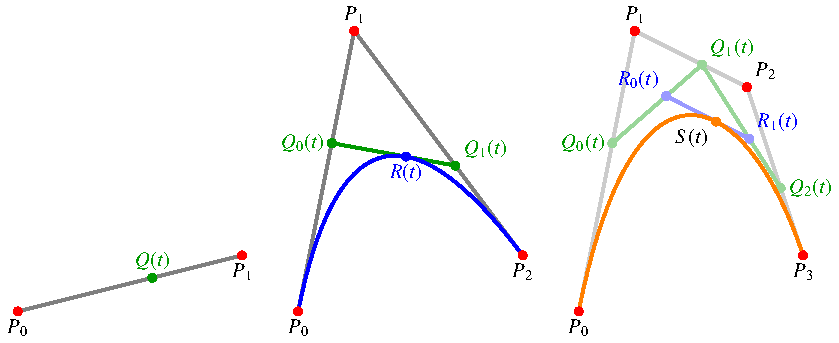
\includegraphics{chapters/30-interpolation/figures/bezier.pdf}
\caption{Bézier-Kurven bis zur Ordnung 3
\label{buch:interpolation:figure:bezier}}
\end{figure}
Die einfachste Verbindung zwischen zwei Punkten $P_0$ und $P_1$ mit
Ortsvektoren $p_0$ und $p_1$ ist eine Strecke, die man mit
\[
\gamma(t) = (1-t)p_0 + tp_1
\]
parametrisieren kann.
Der Tangentialvektor ist bereits bestimmt, er ist
\[
\dot{\gamma}(t) = -p_0 + p_1 = p_1-p_0.
\]
Die zwei Punkte legen den Tangentialvektor bereits fest, man kann
ihn nicht mehr frei wählen.

Kann man eine einfach zu berechnende Kurve finden, die den Punkt $P_0$
mit einem vorgegebenen Geschwindigkeitsvektor verlässt?
Paul de Casteljau hat vorgeschlagen, drei Punkte $P_0$, $P_1$ und $P_2$
zu verwenden und zunächst wie vorhin die Strecken 
\begin{align*}
q_0(t) &= (1-t) p_0 + t p_1 \\
q_1(t) &= (1-t) p_1 + t p_2 
\end{align*}
zu bilden.
Zur Zeit $t=0$ verlässt das erste Segment den Punkt $P_0$ mit der
Geschwindigkeit $p_1-p_0$.
Zur Zeit $t=1$ kommt das zweite Segment im Punkt $P_2$ an mit der
Geschwindigkeit $p_2-p_1$.
Man muss also zwischen $t=0$ und $t=1$ ``vom ersten Segment auf das zweite
wechseln''.
Dazu verbindet man die Punkte $q_0(t)$ und $q_1(t)$ mit einer Strecke und
wähle den Streckenparameter wieder als $t$.
Man erhält so eine Kurve
\begin{align*}
r(t)
&=
(1-t) q_0(t) + t q_1(t)
\\
&=
(1-t) \bigl( (1-t)p_0 + tp_1\bigr)
+
t \bigl( (1-t)p_1 + tp_2\bigr)
\\
&=
(1-t)^2 p_0 + 2t(1-t) p_1 + t^2 p_2.
\end{align*}
Der Geschwindigkeitsvektor zu den Zeiten $t=0$ und $t=1$ ist
\begin{align*}
\dot{r}(t)
&=
-2(1-t)p_0 + (2(1-t)-2t) p_1 + 2tp_2
\\
&=\begin{cases}
-2p_0+2p_1=2(p_1-p_0)&\qquad t=0
\\
-2p_1+2p_2=2(p_2-p_1)&\qquad t=1
\end{cases}
\end{align*}
Die gefundene Kurve verlässt also den Punkt $P_0$ genau in Richtung
auf $P_1$ und kommt im Punkt $P_2$ aus der Richtung von $P_1$ an.
Wir haben also eine quadratische Kurve gefunden, die einen Teil 
der Forderungen erfüllt.

Man nennt diese Kurve eine quadratische {\em Bézier-Kurve} mit
\index{Bézier-Kurve}
{\em Kontrollpunkten} $P_0$, $P_1$ und $P_2$.
\index{Kontrollpunkte}
Der Punkt $P_1$ kontrolliert die Start- und Ankunftsrichtung.

Die beiden Richtungen in Anfangs- und Endpunkten müssen unabhängig
voneinander vorgegeben werden können, wir versuchen daher, die
gleiche Konstruktion mit vier Kontrollpunkten durchzuführen.
Gegeben seien jetzt also die Punkte $P_0,\dots,P_3$.
Dann können wir drei Strecken
\begin{align*}
q_0(t) &= (1-t) p_0 + t p_1 \\
q_1(t) &= (1-t) p_1 + t p_2 \\
q_2(t) &= (1-t) p_2 + t p_3 
\end{align*}
konstruieren.
Die erste hat die ``richtige'' Startrichtung, die letzte die ``richtige''
Ankunfsrichtung.
Kombinieren wir $q_0(t)$ und $q_1(t)$, erhalten wir eine quadratische
Kurve, die vom Punkt $P_0$ mit der richtigen Geschwindigkeit weggeht,
die Kombination von $q_1(t)$ mit $q_2(t)$ liefert eine quadratische
Bézier-Kurve, welche im Punkt $P_3$ mit der richtigen Geschwindigkeit
ankommt.
Wir können also erneut kombinieren:
\begin{equation}
\left.
\begin{aligned}
r_0(t) &= (1-t)q_0(t) + t q_1(t) \\
       &= (1-t)^2 p_0 + 2t(1-t) p_1 + t^2 p_2
\\
r_1(t) &= (1-t)q_1(t) + t q_2(t) \\
       &= (1-t)^2 p_1 + 2t(1-t) p_2 + t^2 p_3
\end{aligned}
\quad
\right\}
\quad\Rightarrow\quad
s(t) = (1-t) r_0(t) + t r_1(t)
\end{equation}
Wir berechnen 
\begin{equation*}
\begin{linsys}{5}
s(t) &=& (1-t) \bigl( (1-t)^2 p_0 &+& 2t(1-t)         p_1 &+& t^2     p_2 &\bigr) & \phantom{\bigr)}\\
     & &                          & & t\bigl( (1-t)^2 p_1 &+& 2t(1-t) p_2 &+& t^2p_3\bigr) \\
     &=& (1-t)^3 p_0 &+& 3t(1-t)^2 p_1 &+& 3t^2(1-t) p_2 &+& t^3 p_3\rlap{.}\phantom{\bigr)}
\end{linsys}
\end{equation*}
Der Tagententialvektor an den Stellen $t=0$ und $t=1$ ist
\begin{align*}
\dot{s}(t)
&=
-3(1-t)^2p_0 + (3(1-t)^2-6t(1-t))p_1 + (6t(1-t)-3t^2)p_2 + 3t^2p_3
\\
\Rightarrow\qquad
\dot{s}(0) &= -3p_0+3p_1 = 3(p_1-p_0)
\\
\dot{s}(1) &= -3p_2 + 3p_3 = 3(p_3-p_2),
\end{align*}
die Kurve verlässt also wie erwartet den Punkt $P_0$ genau in Richtung 
auf $P_1$ und kommt genau aus der Richtung von $P_2$ in $P_3$ an.

Man kann auch die Spline-Funktionen wieder aus der zweidimensionalen
Kurve $s(t)$ rekonstruieren.
Gegeben sind dafür zwei Werte $y_0$ und $y_1$ und die Steigungen $m_0$ und
$m_1$ in den Punkten $x=0$ und $x=1$.
Der Graph des kubischen Polynoms $p(x)$ mit $p(0)=y_0$, $p(1)=y_1$,
$p'(0)=m_0$ und $p'(1)=m_1$ soll jetzt als Bézier-Kurve geschrieben werden.
Dazu müssen die Kontrollpunkte gefunden werden.
Es ist klar, dass $P_0=(0,y_0)$ und $P_3=(1,y_1)$.
Für die inneren Kontrollpunkte muss ein geeigneter $x$-Wert gewählt werden,
also
\[
P_1=
(x_1,y_0+x_1m_0)
\qquad
\text{und}
\qquad
P_2
=
(x_2,y_1-(1-x_2)m_1)
\]
Wählt man $x_1=\frac13$ und $x_2=\frac23$, dann wird
\begin{align*}
x(t)
&=
(1-t)^3\cdot 0 + 3t(1-t)^2\cdot \frac13 + 3t^2(1-t)\cdot \frac23 + t^3\cdot 1
\\
&=
t-2t^2+t^3 + 2t^2 -2t^3 + t^3 = t.
\end{align*}
Mit dieser Wahl ist also $x=t$, so dass das gesuchte Polynom $p(x)=y(x)$ wird:
\begin{align*}
p(x)
=
y(x)
&=
(1-x)^3 y_0
+
3x(1-x)^2\biggl(y_0+\frac13m_0\biggr)
+
3x^2(1-x) \biggl(y_1-\frac13m_1\biggr)
+
x^3 y_1
\\
&=
\bigl((1-x)^3+3x(1-x)^2\bigr)
y_0
+
x(1-x)^2 m_0
-
x^2(1-x) m_1
+
\bigl(3x^2(1-x)+x^3\bigr)
y_1
\\
&=
(1+2x)(1-x)^2 y_0
+
x(1-x)^2 m_0
+
x^2(x-1) m_1
+
x^2(3-2x) y_1.
\end{align*}
Die Koeffizienten von $y_0$, $y_1$, $m_0$ und $m_1$ sind die Polynome
\begin{equation}
\begin{aligned}
y_0:&&
H_0(x)
&=
2x^3-3x^2+1
&\quad&
&m_0:&&
H_0^1(x)
&=
x-2x^2+x^3
\\
y_1:&&
H_1(x)
&=
3x^2-2x^3
&\quad&
&m_1:&&
H_1^1(x)
&=
x^3-x^2
\end{aligned}
\label{buch:bezier:eqn:H}
\end{equation}
Die Polynome \eqref{buch:bezier:eqn:H} stimmen mit den Polynomen überein,
die in \eqref{buch:equation:hermite:h} gefunden worden sind.



